\chapter{Desarrollo}

\section{Map4rdf}
\subsection{Instalación}

Se ha optado por utilizar la máquina Virtual proporcionada en la Wiki del proyecto para minimizar la posibilidad
de incompatibilidades.

\section{GeoKettle}

Desde que se publicó ``A sustainable process and toolbox for geographical linked data generation and
publication: a case study with BTN100'' en 2019, GeoKettle ha dejado de estar soportado. La pagina oficial y de
documentación ya no están disponibles.
Un objetivo de este TFG es dar soporte GeoPackage a GeoKettle. No tiene sentido desarrollar soluciones de
``modernización'' sobre software abandonado. Por tanto, se comenzará actualizando la herramienta.

Algunas funcionalidades de GeoKettle se integraron en PDI directamente y otras desaparecieron. 
Actualmente, el soporte GIS de Pentaho está dentro de PDI Spoon y además hay algunas funcionalidades más en
 el plugin disponible en el marketplace llamado pentaho-gis-plugins. Se actualizará la primera fase a:
\textbf{``replicar la funcionalidad y las transformaciones de GeoKettle + TripleGeo en la suite PDI.''} Si es sencillo,
se considerará también dar soporte a GeoPackage.

Dado que se trata de replicar la funcionalidad anterior, se analizarán las tranformaciones realizadas por el OEG
en el repositorio de GitHub BTN100. Como se puede ver en la figura \ref{fig:spoon-missing-plugins}, partes del
workflow fallan. Es lo que se pretende solucionar.

\begin{figure}[h]
    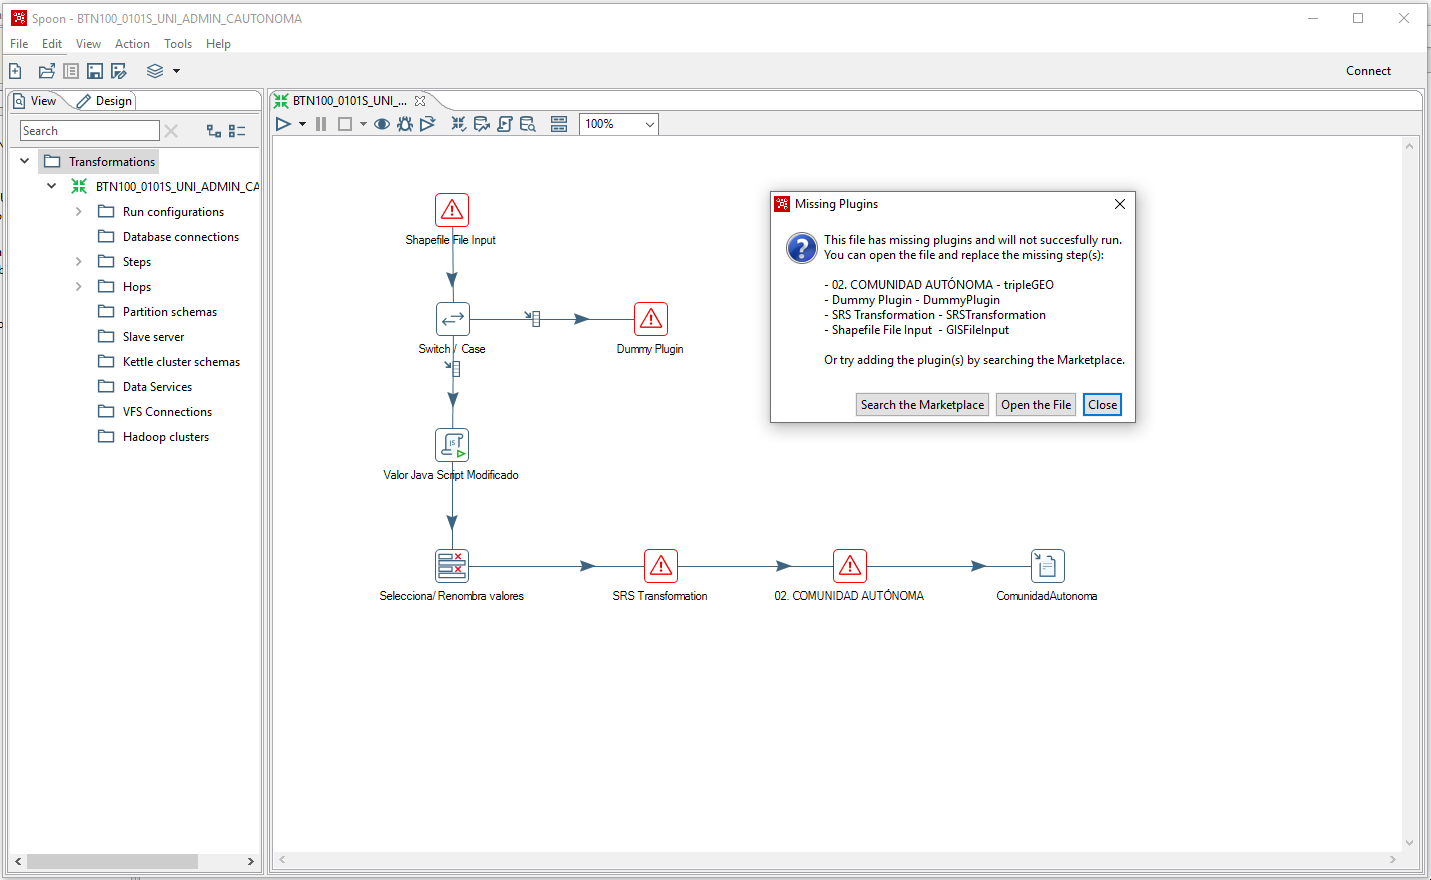
\includegraphics[width=\textwidth]{images/spoon-missing-plugins.png}
    \centering
    \caption{Workflow importado en la nueva suite}
    \label{fig:spoon-missing-plugins}
\end{figure}

\newpage
\subsection{Funcionamiento}

Para poder realizar el ``port'' de GeoKettle a Spoon, primero es necesario entender el funcionamiento y
transformaciones actuales de GeoKettle. Dado que hay poca documentación se realizará ingeniería inversa observando
la entrada y salida de cada paso. Además esta manera se observará mejor el flujo de datos y será más facil añadir
soporte a GeoPackage en el futuro. Como ejemplo se utilizarán los datos de BTN100\_0101S\_UNI\_ADMIN y la
transformación BTN100\_0101S\_UNI\_ADMIN\_CAUTONOMA. La
transformación contiene los siguientes pasos:

\begin{figure}[h]
    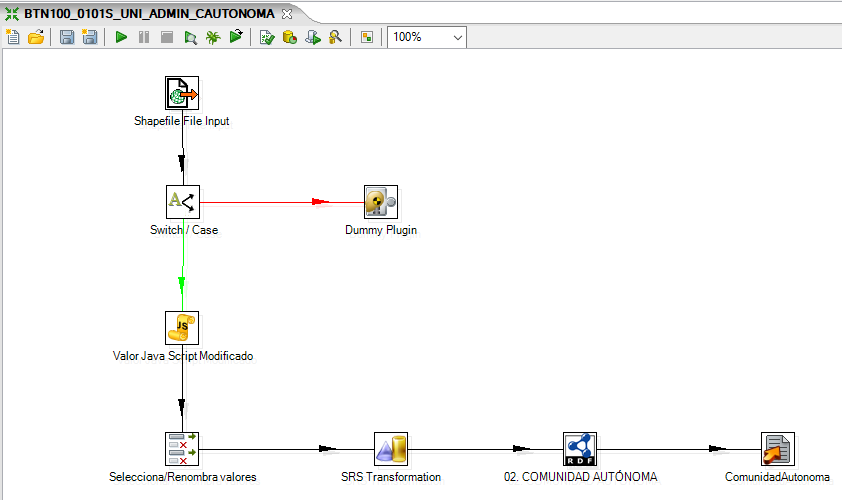
\includegraphics[width=\textwidth]{images/CCAA.png}
    \centering
    \caption{Transformación BTN100\_0101S\_UNI\_ADMIN\_CAUTONOMA}
    \label{fig:CCAA}
\end{figure}


\begin{enumerate}
    \item Shapefile File Input
    \item Switch Case
    \item Dummy Plugin
    \item Valor Java Script Modificado
    \item Selecciona/Renombra valores
    \item SRS Transformation
    \item TripleGeo
    \item Text Output
\end{enumerate}


\subsubsection{Shapefile File Input}

Lee el fichero shapefile.
\begin{enumerate}
    \item \textit{.shp}: Geometría fig.\ref{fig:shapefile}

        \begin{figure}[h!]
            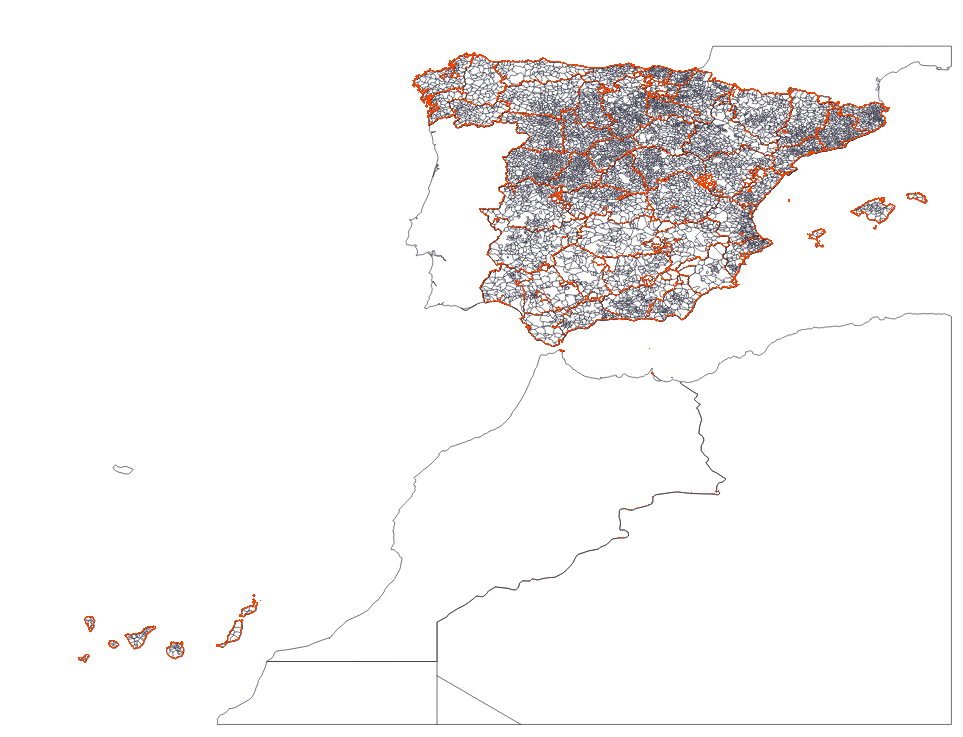
\includegraphics[width=0.7\textwidth]{images/shapefile.png}
            \centering
            \caption{Geometría contenida en el shapefile}
            \label{fig:shapefile}
        \end{figure}

    \item \textit{.dbf}: Datos asociados en columnas fig.\ref{fig:dbf}

        \begin{figure}[h!]
            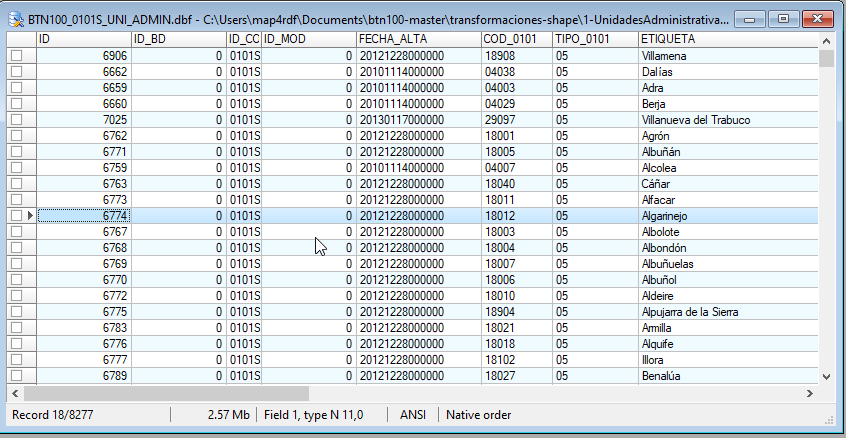
\includegraphics[width=0.7\textwidth]{images/dbf.png}
            \centering
            \caption{Datos columnares dbf asociados a la geometría}
            \label{fig:dbf}
        \end{figure}

    \item \textit{.shx}: Índice para acelerar búsquedas
    \item \textit{.prj}: Sistema de coordenadas
\end{enumerate}

\subsubsection{Switch case}
El switch case se encarga de filtrar y seleccionar las comunidades autónomas, identificadas por el valor 02 del
Campo TIPO\_0101. Si son una CCAA, se envían al paso 4, e.o.c. se envían al paso 3.

\begin{figure}[h]
    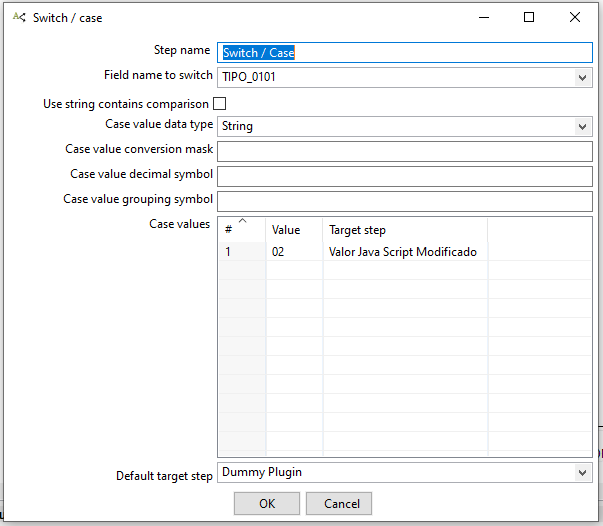
\includegraphics[width=0.7\textwidth]{images/switch.png}
    \centering
    \caption{Paso switch}
    \label{fig:switch}
\end{figure}

\begin{figure}[h]
    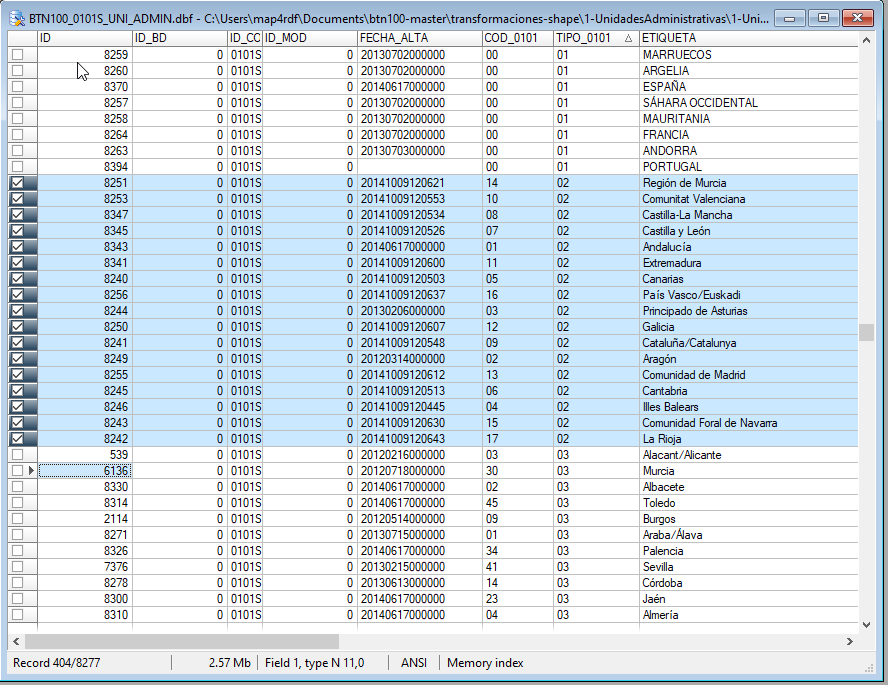
\includegraphics[width=\textwidth]{images/tipo02.png}
    \centering
    \caption{La filas correspondientes a las CCAA}
    \label{fig:tipo02}
\end{figure}

\subsubsection{Dummy Plugin}
No hace ninguna transformación, su propósito es recoger los datos innecesarios del switch.

\subsubsection{Valor Java Script Modificado}
El script cambia el formato de la fecha para facilitar la lectura: de YYYYMMDDHHMMSS a YYYY-MM-DD. También
crea un nuevo campo llamado identificador a partir del campo etiqueta, cambiando espacios por barras bajas, mayúsculas
por minúsculas, quitando tildes y signos de puntuación.

\begin{figure}[h]
    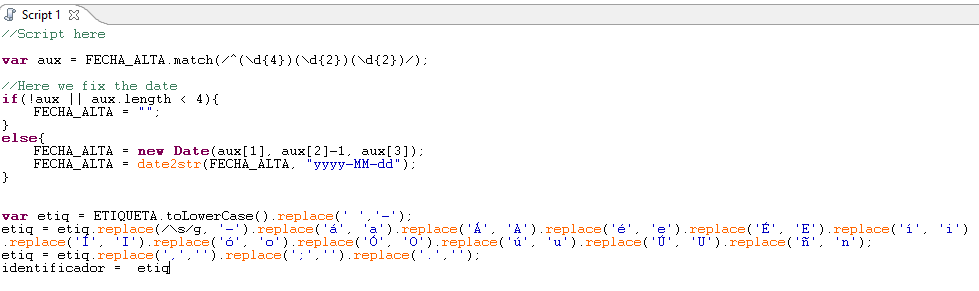
\includegraphics[width=\textwidth]{images/script.png}
    \centering
    \caption{Script Javascript}
    \label{fig:script}
\end{figure}

\begin{figure}[h]
    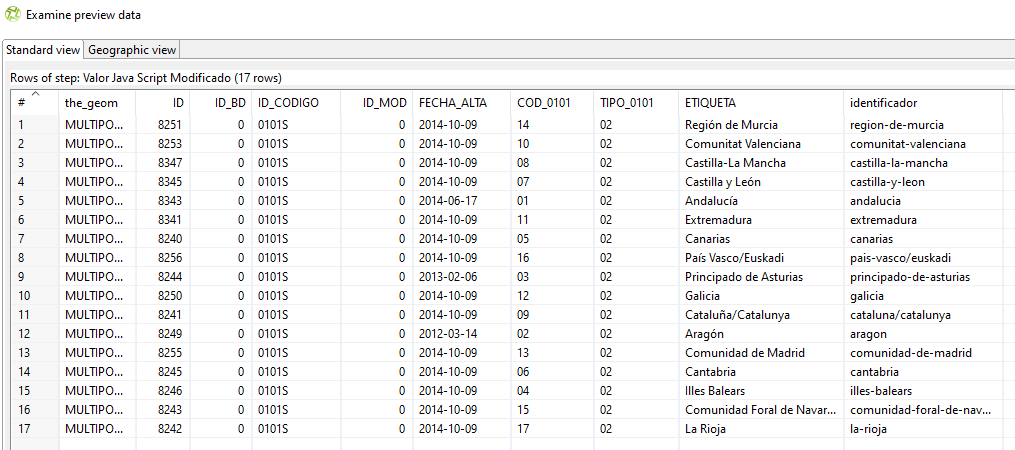
\includegraphics[width=\textwidth]{images/fecha.png}
    \centering
    \caption{Resultado del cambio de formato de fecha}
    \label{fig:fecha}
\end{figure}

\subsubsection{Selecciona/Renombra valores}
Cambia los metadatos de la columna FECHA\_ALTA para que sea reconocida como fecha.
